%*****************************************************************************************
%*********************************** Fourth Chapter **************************************
%*****************************************************************************************

\chapter{Future Work and Discussion}

\ifpdf
    \graphicspath{{Chapter5/Figs/Raster/}{Chapter5/Figs/PDF/}{Chapter5/Figs/}}
\else
    \graphicspath{{Chapter5/Figs/Vector/}{Chapter5/Figs/}}
\fi
\section{Results and Evaluation}\label{sec:ResultsAndEvaluation}

\section{Future Applications}\label{sec:FutureApplications}


\subsection{Medical Applications}\label{sec:MedicalApplications}

\subsection{Scientific Applications}\label{sec:ScientificApplications}

\subsection{Computer Vision Applications}\label{sec:ComputerVisionApplications}


\section{Color Space Algorithm Improvements}\label{sec:ColorSpaceAlgorithmImprovements}
Here we suggest several improvements which could be made to the color space algorithm developed in Chapter 2. The improvements presented herein address generalizing the algorithm to accommodate the characteristics of cameras other than the iPhone's. We consider three adaptations; one to allow for multi-spectral cameras, another to allow for cameras which do not have a fixed white point, and a third to handle RAW images captured from the CCD without the iPhone's pre-processing. In practice, these three adaptations need to be combined. Hopefully it shouldn't be too difficult to imagine how this could be done, but in terms of practically proceeding, each one would need to be tackled individually first.

\subsection{Generalizing the Rotation}\label{sec:GeneralizingTheRotation}
In Chapter 2, we derived an expression for a rotation matrix consisting entirely of integers which rotates the RGB pixel values into a custom color space with a luminosity axis and two chromatic axes. The orientation of the chromatic axes is specified using a free rotation $\theta$ about the luminosity axis. The only restriction on the free parameter $\theta$ is that which results from the requirement for the matrix to consist entirely of integer values within a specific range. The question remains: is it possible to achieve a similar result without restricting one of the axes?

In this work, we assumed that an 8-bit per-channel value of $(255, 255, 255)$ corresponds with white. This, however is a result of the pre-processing on the iPhone. Extending this work to other devices or accessing the iPhone's RAW camera feed, it may be desirable to use a different point for the camera's white point. Another reason is to adjust for local ambient light conditions; it is common in digital photography to choose a pixel value from a reference white object to set a white point for the image, allowing a color correction to be performed.

An arbitrary rotation is determined by three angles, and so it's conceivable that the work of Chapter 2 (Section \ref{sec:ConstructingANewColorSpace}) could be repeated for this arbitrary rotation. Whilst it may be possible, an alternative approach may be preferable given the complexity of the general rotation equations. First we assume that the solution exists, then form an initial guess at the solution by quantizing the floating point representation of the matrix. Next, we find the maximum error produced by our approximate quantized rotation by rotating the corners of the RGB cube and comparing the results, then numerically search around this approximation for improvements. The question that remains is what search area should be included.

<math here>

Because the general rotation matrix can be split into the product of three individual matrices, each of which is dependent on only one of the three free parameters, the work in Section \ref{sec:ConstructingANewColorSpace} could be repeated relatively straightforwardly for each of these three individual matrices, and from this --- for a given quantization criteria --- a minimum and a maximum angle step size (Figure \ref{fig:PtbToChan}). If we have for the separate matrices a minimum and a maximum step size, it's a reasonable idea to search around our initial approximation in steps of the minimum step size to either side out to a maximum distance of the maximum step size. For each of the three angles, we search within a cube with sides defined by the maximum step sizes for each of those rotation matrices. On a cubic grid defined by their minimum step sizes. The result of this is that there is a relatively small set of possible optimized choices. Although this is not solving the problem to the same degree that was done in \ref{sec:ConstructingANewColorSpace}, where we reduced it to a mathematical function, it provides a practical way of achieving the same results without excessive computational effort in the setup. 

\subsection{Multi-Channel Color Spaces}\label{sec:MultiChannelColorSpaces}

As mentioned in Chapter 1, the RGB color space is an approximation to the full spectrum of light. However, cameras which are not confined to the three-channel approximation are becoming commercially available (Figure \ref{fig:MultiSpectralCameras}); such a multi-channel image contains far more information about the objects in frame. So where the camera is being used for computer vision tasks where the objective is not to produce a pretty picture to present to the human eye, this allows the chromatic space to discriminate between different objects and surfaces in ways which are unseen by the standard RGB camera point of view.

\begin{figure}
  \centering
  \begin{tabular}{cc}
  \subfloat[Triwave EC701.]{
    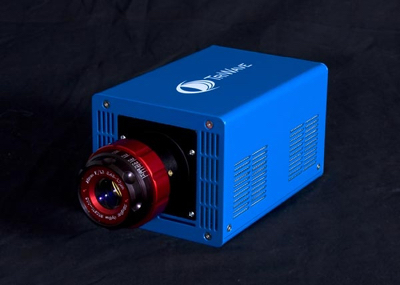
\includegraphics[width=.49\textwidth]{Chapter5/Figs/multispec-triwave.jpg}
    }&
  \subfloat[HyperCam by University of Washington and Microsoft Research.]{
    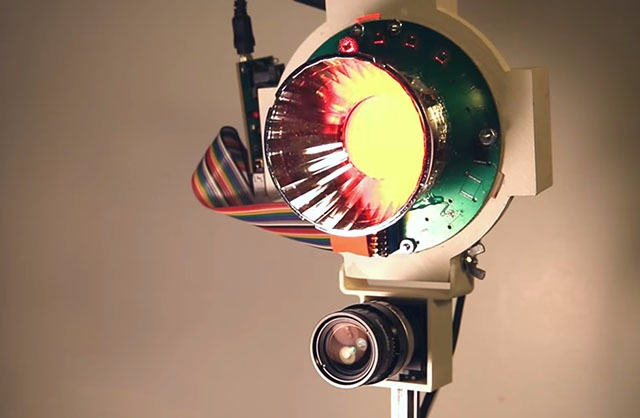
\includegraphics[width=.49\textwidth]{Chapter5/Figs/multispec-hypercam.jpg}
    } \\
    \multicolumn{2}{c}{
    \subfloat[Optec multi-spectral camera.]{
        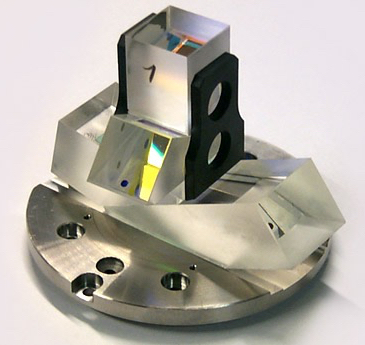
\includegraphics[width=.49\textwidth]{Chapter5/Figs/multispec-optec.jpg}
    }
    }
  \end{tabular}
  \caption{A variety of multi-spectral cameras currently in use.}
  \label{fig:MultiSpectralCameras}
\end{figure}

The basic design of these multi-spectral cameras is essentially the same as for the RGB cameras where the spectrum of light on each point in the scene (roughly speaking, see Chapter 1) is represented by a combination of Gaussians, the only difference being we have more Gaussians. Each channel can therefore be considered an orthogonal axis in a multi-dimensional color space. The multi-dimensional color space contains a point which corresponds to white, so it is just as possible to construct a color space with a luminosity axis and $n-1$ chromatic axes for an $n$-channel image. Transformation to this color space is defined by a multi-dimensional rotation; this rotation could be optimized in a similar way to that presented in Chapter 2. However, our requirement in Chapter 2 was that the immediate result of the rotation would fit into a data type no more than twice the bit depth of each channel. An $n$-channel color space will be rotated by an $n$ x $n$ rotation matrix; if we have $m$ bits per channel and the quantized rotation matrix is expressed in $l$-bit integers, the result is $l + m + (n-1) \leqslant 2m$. For the larger values of $n$, the rotation matrix would have to be expressed in smaller data types, so aside from special rotation angles which just happen to produce integer rotation matrices, it's unlikely that our criterion can be met. So for multi-channel images to still be able to use integer rotation matrices, the target data type will undoubtedly have to be significantly larger. 

\subsection{Using the RAW Image From the Camera}\label{sec:UsingTheRAWImageFromTheCamera}
The RAW camera image contains all the information captured by the camera, but without any pre-processing. Individual CCDs have different sensitivities in each of their channels, and so the corresponding bit depth of each channel may actually vary. This is likely to be the case for the iPhone's camera as we found in Chapter 3 that certain RGB values appear to be inaccessible. These inaccessible values also appear to be relatively evenly-spread throughout the RGB cube, which produced what we referred to as "speckling" in the statistics gathered in Chapter 3 as seen in Figure \ref{fig:Despeckle_the_Bins}. 

A possible explanation for this is that one or more of the iPhone camera's channels are not truly captured at an 8-bit depth, but a smaller range of values which the CCD actually captures is stretched to fit the full 8-bit range. It is also entirely possible that one or more of the channels may actually be captured at a higher bit depth than 8-bit. But in terms of the algorithm, we now need to allow each channel in the source to have a variable bit depth. This will affect several things; it changes the integer range of allowed values in a rotation matrix and the algorithm for determining the optimal angle could be adapted by weighting the channels appropriately. But otherwise, adapting to a RAW camera image should be relatively straightforward.

\section{Implementation Improvements}\label{sec:ImplementationImprovements}

\subsection{An Empirical WoBo Algorithm}\label{sec:EmpicialWoBoAlgorithm}
The White-out Black-out algorithm outlined in \ref{sec:WhiteoutAndBlackout} uses theoretical values based on the extent of the data type used to store the RGB image. Looking at the empirical results presented in Figure \ref{fig:WhitePoint}, there's more to the WoBo behavior than simply saturating the data type; the performance of the CCD changes with overall ambient light, and the pre-processing performed on the device also has an effect which takes the pixel values away from the naive data point values using the data type extent. 

Although it may be possible to reverse-engineer both the pre-processing and CCD characteristics simultaneously, this would be a difficult task at best. However, if for a device we were able to obtain the RAW image from the CCD, then repeatedly performing empirical tests, such as those performed to generate Figure \ref{fig:WhitePoint}, the CCD characteristics could be obtained. If we know how the CCD detects objects of a certain color under different ambient luminosities, then a more nuanced algorithm can be used to determine if a certain pixel value has suffered from white-out or black-out.

\subsection{Auto-Adjusting the Variance}\label{sec:AutoAdjustingTheVariance}
The algorithm presented in Chapter 4 uses a reference image to float the mean, yet algorithm makes no attempt to adjust the variance to local ambient light conditions. This is found to work well, however it was initially found that using a standard deviation 2.3 times larger than the value found in Chapter 3 produced better results. (See Figure \ref{fig:RelaxedSigma}.) Although the algorithm was tested against a selection of background colors which are notably close to skin colors were avoided. For practical applications, it may therefore be useful to use a value for the standard deviation close to that used in Chapter 3.

The image is chosen to be included in this document were taken against a green background because that gave the cleanest results; a value of 2.3$\sigma$ produced good results in this ideal background condition, so we'll choose 2.3 as the overall upper limit and 1$\sigma$ as the overall lower limit. We have a reference image where we have a good idea that there is a finger, and a portion of that finger is within a known frame, so the lower criteria is that nearly all, if not all, the pixel values within that frame are categorized as skin using the new value for the standard deviation, so for a choice between 1$\sigma$ and 2.3$\sigma$, we can "score" the choice as follows:

\begin{enumerate}
\item The proportion of pixels within the known skin region successfully classified as skin.
\item The number of edge points found using the Filament fill algorithm which are classified as bad edge points which also lie outside the approximated digit edge.
\item The number of edge points found by Filament fill which are classified as bad edge points, but which lie within the edges of the digit.
\end{enumerate}

So, a score where measure 1 is too low suggests that $\sigma$ should be increased, as pixel values which we know to be skin are classified as not skin; if measure 2 is too high, then we need to reduce the value of $\sigma$; and if measure 3 is too high, then we need to increase the value of $\sigma$.

This suggests a way that an algorithm could be developed which appropriately adjusts the value of $\sigma$ striking a compromise between false negatives and false positives. The actual values, thresholds and criteria used can best be determined empirically.

One way of proceeding may be to combine the three measures by taking the weighted product of measures 2 and 3 with the weighted reciprocal of measure 1. We combine the measures in this fashion and minimize the result with respect to $\sigma$.

\subsection{Statistics Gathering Method for the App}\label{sec:StatisticsGatheringMethod}
Given that, in the implementation, we have "floated" the mean and "relaxed" the standard deviation, and above, a method is suggested for adaptively adjusting the standard deviation, it is natural to consider whether the app can handle all the work from Chapter 3. Collecting the statistical model following Chapter 3 is entirely possible, as at no point is any human intervention necessary. However, the Chapter 3 methodology requires that a set of images are captured against a uniform, highly chromatically-contrasting background, which is not a practical or interesting extension to the app.

An interesting possibility is whether the work of Chapter 3 can be somewhat replicated using the same reference image which is used by the app to float the mean and build the initial fingertip model. The difficulties with this idea are the same two difficulties faced by most statistics-gathering methods; sample size and selection bias. To address the first difficulty, we've seen that the number of pixels within the frame which correspond to skin is sufficiently large to usefully adjust the mean of the distribution. This suggests that the sample size should not be a significant problem. Selection bias, on the other hand, comes from asking the user to select a portion of their finger which they consider to be most skin-like; this is not an explicit request of the user, but an implicit request, i.e. when asking a person to supply a sample of skin, they will supply the most skin-like sample they can. This selection bias will likely exclude the edges of the digit, strong features and poorly-lit portions of the skin. As a result, while the mean almost certainly will be fine, the variance will be narrow. So, it's easy to imagine using techniques suggested for auto-adjusting the variance (Section \ref{sec:AutoAdjustingTheVariance}) to make the distribution more inclusive.

One final refinement suggests itself at this point; the resulting color space can be used to model the fingertip and mask the image such that only on-digit pixels are present. In doing this, we now have a broader sample set of pixel values which don't suffer from selection bias. These pixel values could be passed back through the statistical model algorithm to produce a skin chromatic model which is less susceptible to human input.

\subsection{Improved ICWaS Alignment}\label{sec:ImprovedICWaSAlignment}

\subsection{More Designed Metric for Mechanical Stress}\label{sec:MoreDesignedMetricForMechanicalStress}
The metric method which is very briefly presented at the end of Chapter 4 (see Figures \ref{fig:ICWaSResultJSkin}, \ref{fig:ICWaSResultFSkin} and \ref{fig:ICWaSResultNSkin}) relies on a pixel-to-pixel comparison; it is well known that pixel-based methods are unreliable for detecting movement, and our mechanical stress measurement relies on detecting the flow of blood. The metric should therefore account for neighboring pixels. 

There are many possible methodologies for detecting movement which would improve the pixel-based method of Chapter 4. Mechanical stress tends to move pooled blood from one area to another within the stressed tissue. The upshot of this is that as one portion of the image loses blood, another gains it. This is different to the circulatory blood, which is pumped in through the arteries and capillaries and flows out through the veins. A better metric may be to compare blobs in the negative and positive chromatic difference images. To be clear, the algorithm would find blobs using a negative thresholding and a positive thresholding; the largest blobs in each of these spaces would be considered good indicators of pooled blood flow.

Another possibility arises from incidental observations of the pooled blood flow images; for each individual's digit, the pooled blood flow pattern is fairly consistent under similar mechanical stress conditions. This suggests that it may be possible to construct a blood flow model for a given digit. Regarding the app, we can imagine generalizing the reference image idea to asking the user to press on a surface several times, allowing the blood flow model to be generated for that digit.

\section{Conclusion}\label{sec:ConclusionCh5}

The finger press algorithm is really a simple application to demonstrate the viability of detecting blood movement using a standard camera on a mobile device. Many previous authors have dismissed using bespoke color spaces for such applications simply because the color space transform itself is computationally intensive and significantly loses information when applied using standard, off-the-library-shelf color spaces. It's fundamentally difficult to use with the loss of information, with white-out and black-out, and the computational intensity right at the front of the algorithm have meant that such techniques have seen little use.

It is hoped that, with the rigorous optimization of the transform itself --- which is considered in great and incredibly tedious detail in chapter 2 --- that these color spaces can see greater application in the future, although it's recognized that the level of attention that's currently required to make the routine as efficient at the one designed herein will likely be beyond the patience of many practitioners, some of whom are medical professionals and not computer scientists. Also, it is hoped that the work presented here has addressed the concerns about the loss of information associated. This surely must be the case because the color space transform is designed not to lose any information from the RGB color space.

Finally, the use of a Gaussian model for the skin color space has been the source of much debate; some authors insist that the Gaussians be extended to the three-dimensional space, but hopefully it can be seen from this work that a luminosity Gaussian distribution is an artifact due to white-out and black-out, and so is not necessary. The potential gains of using such a luminosity distribution would appear to be gained using the 2-bit Canny edge detection algorithm outlined in~\ref{sec:ImprovedContourDetection}.

The color space algorithm has many possible future applications as an aid to diagnostics, however specialist cameras will always outperform in this area. Also, mechanical stress is not limited to the end of the fingers; knuckles significantly whiten when flexed, so the color space could aid in hand posture work, as would the Canny edge detection methods --- although not presented here during the design of the algorithm --- it was striking how clearly other hand features presented themselves. For instance, it was very tempting to attempt to attach a feature descriptor to the perpendicular creases in the knuckles.

Although not presented here, the majority of the time and effort involved in producing this work went into the furthering of the OpenCV library, which is an open source project hosted on GitHub. The reason this occupied so much of the time is because, at the start of this project, there was no working implementation for iOS. Additionally, the new C++11 standard was released and many of the associated libraries were upgraded, as is so oftenthe case with computer science projects, a significant amount of time had to be dedicated to actually making the code and the libraries work on the selected device appropriately. Probably the most significant contribution this project has made to the library is the extension of the internal data types, which were necessary both for the C++11 standard and the 2-bit and 4-bit types which allowed for the optimization of many of the heavy-duty routines.

As for the finger pressure detector, it could be extended to detect the whole hand and to track the individual digits; with work and some machine learning algorithms, it should be possible to enable the app to measure the degree of pressure, which would be ideally suited to a project such as a paper piano, or perhaps even an augmented reality keyboard.